\subsection{Powerset monad}

\begin{frame}{Probability Monads}
	\begin{example}[Powerset Monad]
		$\cat{Set}$ is cartesian monoidal $\Rightarrow$ morphisms are deterministic
		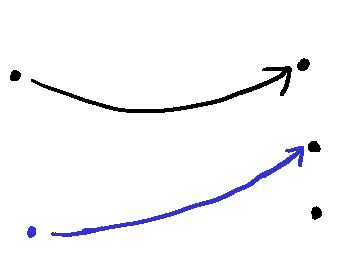
\includegraphics[scale=0.4]{part2/Figures/morphisms_set}
%		\pause 
		\begin{equation*}
		\begin{split}
		\text{Powerset monad} ~
		2^{\bullet} : \cat{Set} &\to \cat{Set}, \quad \\
		X &\mapsto 2^X := \{ M \subseteq X \}
		\end{split}
		\end{equation*}
%		\pause
		\begin{minipage}{0.69\linewidth}
			Kleisli category $\cat{Set}_{2^{\bullet}}$ has morphisms: 
			\begin{equation*}
			\begin{split}
				f : X &\to 2^Y	
				\quad \text{i.e.~}
				f(x) \subseteq Y
			\end{split}
			\end{equation*}
			As Pablo stated: describes \emph{possibility}
	\end{minipage}
	\begin{minipage}{0.3\linewidth}
		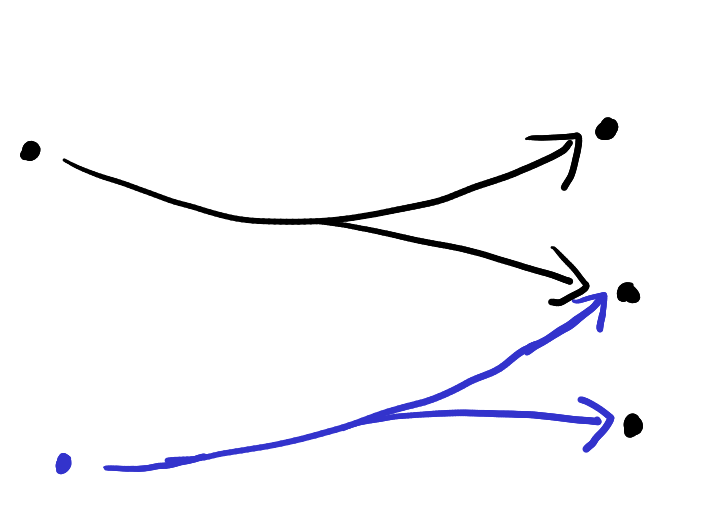
\includegraphics[scale=0.4]{part2/Figures/morphisms_poss}
	\end{minipage}
%	Problem: \enquote{impossibility}
%	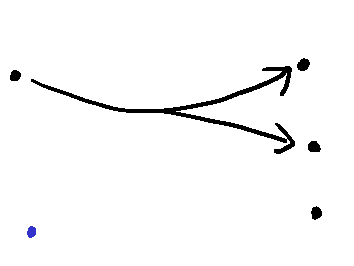
\includegraphics[scale=0.4]{part2/Figures/morphisms_no_poss}
	\end{example}
\end{frame}

\begin{frame}{Probability Monads}
	\begin{example}[Powerset Monad]
%		$\cat{Set}$ is cartesian monoidal $\Rightarrow$ morphisms are deterministic
%		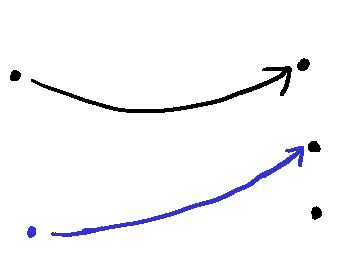
\includegraphics[scale=0.4]{part2/Figures/morphisms_set}
%%		\pause 
%		\begin{equation*}
%		\begin{split}
%		\text{Powerset monad} ~
%		2^{\bullet} : \cat{Set} &\to \cat{Set}, \quad \\
%		X &\mapsto 2^X := \{ M \subseteq X \}
%		\end{split}
%		\end{equation*}
%%		\pause
		\begin{minipage}{0.74\linewidth}
			Problem: Kleisli category $\cat{Set}_{2^{\bullet}}$ has morphism: 
			\begin{equation*}
			\begin{split}
			f : X &\to 2^Y	
			\quad \text{with} \quad
			f(x_i) = \emptyset
			\end{split}
			\end{equation*}
%			this describes \emph{im}possibility
		\end{minipage}
		\begin{minipage}{0.25\linewidth}
			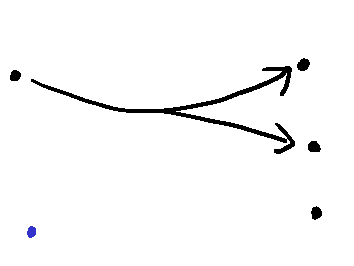
\includegraphics[scale=0.4]{part2/Figures/morphisms_no_poss}
		\end{minipage}
		\pause
		\begin{equation*}
			\tikzfig{counitality_l}
			= 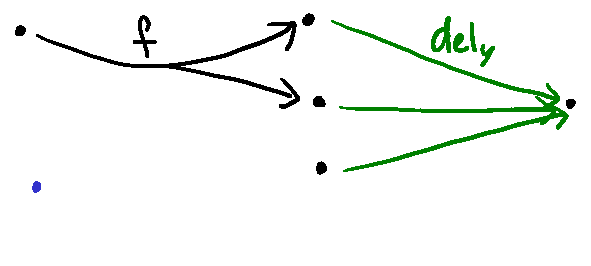
\includegraphics[scale=0.3]{part2/Figures/morphisms_no_poss_composed_1}
			= 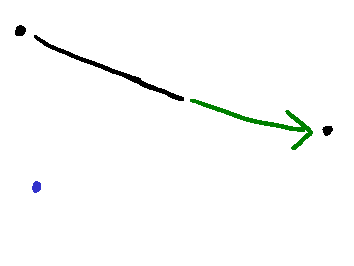
\includegraphics[scale=0.3]{part2/Figures/morphisms_no_poss_composed_2}
			\neq 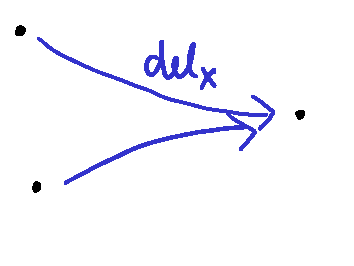
\includegraphics[scale=0.3]{part2/Figures/morphisms_no_poss_composed_3}
			= \tikzfig{counitality_r}
		\end{equation*}
%		\pause
		$\Rightarrow$ $\cat{Set}_{2^{\bullet}}$ is \emph{not} Markov! 
%		\pause
%		\\ $\rightsquigarrow$ adjust monad:
		\begin{equation*}
		\begin{split}
				\rightsquigarrow \text{adjust monad} \quad
				T : \cat{Set} &\to \cat{Set}, \quad \\
				X &\mapsto 2^X - \emptyset
		\end{split}
		\end{equation*}
%		\pause
		$\Rightarrow$ $\cat{Set}_{T} =: \cat{Poss}$ is Markov. \pause With uncertainty.
	\end{example}
\end{frame}